% ============================================================
%  Module 1 — The Invisible Hand
%  From Smith to Simulation · University of Edinburgh
% ============================================================
\documentclass[aspectratio=169, 10pt]{beamer}
\usetheme{metropolis}

% --- Edinburgh colours ----------------------------------------
\definecolor{UoERed}{HTML}{7A2318}
\definecolor{UoEGold}{HTML}{B8860B}
\definecolor{CodeBG}{HTML}{F7F3ED}
\definecolor{CodeFrame}{HTML}{D5C9B1}

\setbeamercolor{palette primary}{bg=UoERed, fg=white}
\setbeamercolor{frametitle}{bg=UoERed, fg=white}
\setbeamercolor{title separator}{fg=UoEGold}
\setbeamercolor{progress bar}{fg=UoEGold, bg=UoEGold!20}
\setbeamercolor{alerted text}{fg=UoERed}
\setbeamercolor{block title}{bg=UoERed!15, fg=UoERed}
\setbeamercolor{block body}{bg=UoERed!5}

% --- Packages -------------------------------------------------
\usepackage[T1]{fontenc}
\usepackage{lmodern}
\usepackage{amsmath, amssymb, mathtools}
\usepackage{listings}
\usepackage{graphicx, booktabs}
\usepackage{tikz}
\usetikzlibrary{arrows.meta, positioning, calc, decorations.pathreplacing}
\usepackage{hyperref}
\hypersetup{colorlinks=true, linkcolor=UoERed, urlcolor=UoERed!70!black}
\setbeamertemplate{navigation symbols}{}

\lstset{
  language=Python,
  basicstyle=\ttfamily\scriptsize,
  keywordstyle=\color{UoERed}\bfseries,
  commentstyle=\color{gray}\itshape,
  stringstyle=\color{UoEGold},
  backgroundcolor=\color{CodeBG},
  frame=single,
  rulecolor=\color{CodeFrame},
  numbers=none,
  breaklines=true,
  showstringspaces=false,
  tabsize=4,
  xleftmargin=4pt, xrightmargin=4pt,
  aboveskip=6pt, belowskip=4pt,
}

% Section title pages
\AtBeginSection[]{
  \begin{frame}
    \vfill\centering
    \usebeamerfont{title}\insertsectionhead\par
    \vfill
  \end{frame}
}

% ---- Title ---------------------------------------------------
\title{Module 1 --- The Invisible Hand}
\subtitle{Adam Smith and Market Equilibrium}
\author{Dr Juan Zurita}
\institute{From Smith to Simulation\\
The University of Edinburgh~$\cdot$~School of Economics}
\date{}

\begin{document}

% =============================================================
\maketitle
% =============================================================

% -------------------------------------------------------------
\section{Part I --- The History}
% -------------------------------------------------------------

\begin{frame}{Edinburgh, 1776}
\begin{columns}[T]
\column{0.55\textwidth}
\begin{itemize}
  \item March 1776: a retired professor of moral philosophy publishes\\
        \textit{An Inquiry into the Nature and Causes of the Wealth of Nations}.
  \item \textbf{Adam Smith} (1723--1790) had spent ten years writing it ---
        mostly in his mother's house in Kirkcaldy.
  \item The book that \alert{founded modern economics}.
\end{itemize}
\column{0.4\textwidth}
\begin{block}{Edinburgh Connection}
Smith attended the University of Edinburgh before Oxford (which he found
``vastly inferior''). He spent his last years at \textbf{Panmure House}
on the Canongate --- you can still visit it today.
\end{block}
\end{columns}
\end{frame}

\begin{frame}{What Smith Was Arguing Against}
\begin{block}{Mercantilism}
  The dominant economic doctrine of 1776:
  \begin{itemize}
    \item National wealth $=$ hoarding gold and silver.
    \item Governments set tariffs, granted monopolies, banned exports.
    \item The economy was something to be \textit{directed from above}.
  \end{itemize}
\end{block}
\vspace{0.5em}
Smith's radical claim: government direction is not only \textbf{unnecessary} but
\textbf{counterproductive}.
\end{frame}

\begin{frame}{The Invisible Hand}
\begin{center}
\textit{``It is not from the benevolence of the butcher, the brewer,\\
or the baker that we expect our dinner, but from their\\
regard to their own interest.''}\\[4pt]
--- Adam Smith, \textit{The Wealth of Nations}, Book~I, Ch.~2
\end{center}
\vspace{1em}
\begin{itemize}
  \item Individuals pursuing self-interest $\Rightarrow$ socially beneficial outcomes.
  \item No one plans the economy, yet bread gets baked, shoes get made,\\
        goods reach those who want them.
  \item The mechanism: \alert{prices and markets} coordinate decisions.
\end{itemize}
\end{frame}

\begin{frame}{The Scottish Enlightenment}
Smith was part of one of the most extraordinary intellectual circles in history:
\vspace{0.5em}
\begin{description}
  \item[\textbf{David Hume}] Philosopher, historian, Smith's closest friend.
        Radical empiricism shaped Smith's method.
  \item[\textbf{Joseph Black}] Chemist who discovered latent heat,
        right here at Edinburgh.
  \item[\textbf{James Hutton}] Geologist who realised the Earth was
        unimaginably old.
  \item[\textbf{Adam Ferguson}] Coined the phrase ``civil society.''
\end{description}
\vspace{0.5em}
Shared commitment: understand the world through \textbf{observation and
systematic reasoning}, not appeals to authority.
\end{frame}

\begin{frame}{Supply, Demand, and the Natural Price}
Smith distinguished:
\vspace{0.5em}
\begin{columns}[T]
\column{0.48\textwidth}
\begin{block}{Natural Price}
  What a good costs to produce (wages, rent, profit at ``ordinary'' rates).
\end{block}
\column{0.48\textwidth}
\begin{block}{Market Price}
  What the good actually sells for, driven by the balance of supply and demand.
\end{block}
\end{columns}
\vspace{1em}
\textit{``The natural price \ldots\ is, as it were, the central price,
to which the prices of all commodities are continually gravitating.''}\\[4pt]
\hfill--- \textit{WN}, Book~I, Ch.~7
\end{frame}

\begin{frame}{The Gravitational Logic}
\begin{center}
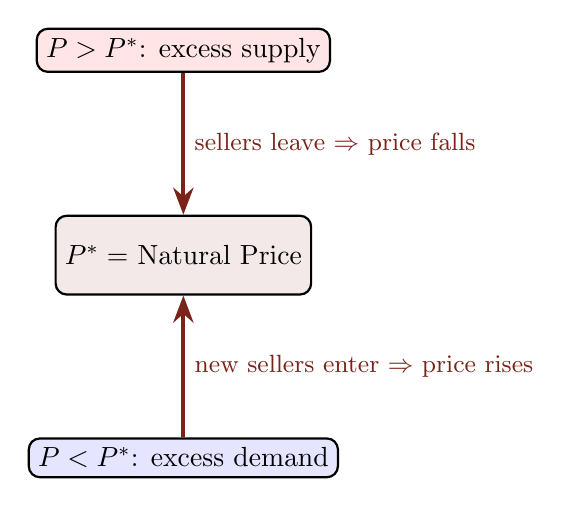
\begin{tikzpicture}[>=Stealth, thick, scale=0.9]
  \node[draw, rounded corners, fill=UoERed!10, minimum width=3cm, minimum height=1cm]
    (eq) {$P^* = $ Natural Price};
  \node[above=1.8cm of eq, draw, rounded corners, fill=red!10] (high)
    {$P > P^*$: excess supply};
  \node[below=1.8cm of eq, draw, rounded corners, fill=blue!10] (low)
    {$P < P^*$: excess demand};
  \draw[->, line width=1.5pt, UoERed] (high) -- node[right, font=\small]
    {sellers leave $\Rightarrow$ price falls} (eq);
  \draw[->, line width=1.5pt, UoERed] (low) -- node[right, font=\small]
    {new sellers enter $\Rightarrow$ price rises} (eq);
\end{tikzpicture}
\end{center}
\vspace{0.5em}
The market \textbf{self-corrects} --- without anyone directing it.\\
This is the invisible hand at work.
\end{frame}

% -------------------------------------------------------------
\section{Part II --- The Computation}
% -------------------------------------------------------------

\begin{frame}[fragile]{Setting Up}
\begin{lstlisting}
import numpy as np
import matplotlib.pyplot as plt
from scipy.optimize import fsolve
\end{lstlisting}
\vspace{0.5em}
\begin{itemize}
  \item \texttt{numpy} --- numerical arrays and operations
  \item \texttt{matplotlib} --- plotting
  \item \texttt{fsolve} --- numerical root-finder\\
        (the computational equivalent of Smith's ``gravitating'' price)
\end{itemize}
\end{frame}

\begin{frame}{Supply and Demand as Functions}
Edinburgh's oat market, c.\,1770:
\vspace{0.5em}
\begin{align*}
  Q^D(P) &= a - bP = 200 - 4P  & &\text{(Demand)} \\[4pt]
  Q^S(P) &= c + dP = 20 + 3P   & &\text{(Supply)}
\end{align*}
\vspace{0.3em}
\begin{itemize}
  \item Demand slopes down: higher price $\Rightarrow$ fewer buyers.
  \item Supply slopes up: higher price $\Rightarrow$ more sellers.
  \item Where do they cross? That is the equilibrium.
\end{itemize}
\end{frame}

\begin{frame}[fragile]{Defining the Market in Python}
\begin{lstlisting}
# Parameters for Edinburgh's oat market
a, b = 200, 4   # demand: Q_D = a - b*P
c, d = 20,  3   # supply: Q_S = c + d*P

def demand(P):
    return a - b * P

def supply(P):
    return c + d * P
\end{lstlisting}
\vspace{0.5em}
At $P = 20$ shillings:
\begin{itemize}
  \item $Q^D = 200 - 4(20) = 120$ bushels demanded
  \item $Q^S = 20 + 3(20) = 80$ bushels supplied
  \item \alert{Shortage} of 40 bushels $\Rightarrow$ price rises
\end{itemize}
\end{frame}

\begin{frame}{Plotting the Market}
\begin{center}
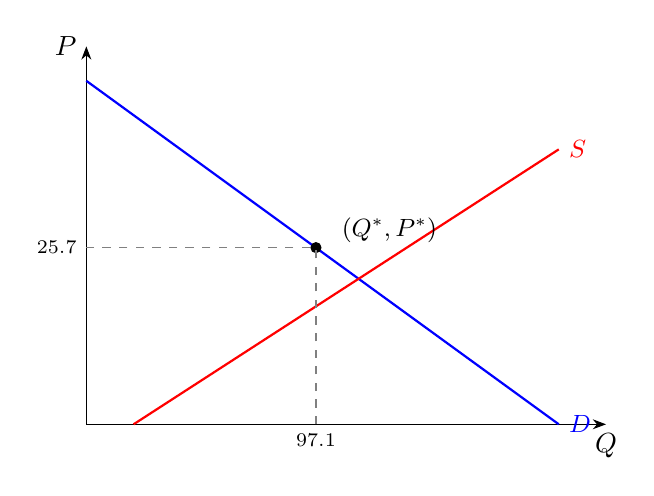
\begin{tikzpicture}[scale=0.6, >=Stealth]
  % Axes
  \draw[->] (0,0) -- (11,0) node[below] {$Q$};
  \draw[->] (0,0) -- (0,8) node[left] {$P$};
  % Demand: P = (200 - Q)/4 = 50 - Q/4  =>  at Q=0, P=50; at Q=200, P=0
  % Scale: Q axis 0-200 => 0-10; P axis 0-55 => 0-8
  % Demand line: (0, 7.27) to (10, 0)  [P=50 to P=0]
  \draw[thick, blue] (0, 7.27) -- (10, 0) node[right, font=\small] {$D$};
  % Supply: P = (Q - 20)/3  =>  at Q=20 P=0; at Q=200 P=60
  % (1, 0) to (10, 5.82)
  \draw[thick, red] (1, 0) -- (10, 5.82) node[right, font=\small] {$S$};
  % Equilibrium: P* = 180/7 = 25.71, Q* = 200 - 4*25.71 = 97.14
  % Scaled: Q*=4.86, P*=3.74
  \filldraw (4.86, 3.74) circle (3pt);
  \draw[dashed, gray] (4.86, 0) -- (4.86, 3.74) -- (0, 3.74);
  \node[right, font=\small] at (5.2, 4.1) {$(Q^*, P^*)$};
  \node[below, font=\scriptsize] at (4.86, 0) {$97.1$};
  \node[left, font=\scriptsize] at (0, 3.74) {$25.7$};
\end{tikzpicture}
\end{center}
\vspace{0.3em}
Convention (Marshall): price on $y$-axis, quantity on $x$-axis.
\end{frame}

\begin{frame}{Excess Demand}
\begin{equation*}
  ED(P) = Q^D(P) - Q^S(P)
\end{equation*}
\vspace{0.3em}
\begin{itemize}
  \item $ED(P) > 0$: \textbf{shortage} --- buyers want more than sellers offer.
        Price tends to \textit{rise}.
  \item $ED(P) < 0$: \textbf{surplus} --- sellers offer more than buyers want.
        Price tends to \textit{fall}.
  \item $ED(P) = 0$: \alert{equilibrium}.
\end{itemize}
\vspace{0.5em}
Smith's gravitational logic, expressed as a function whose \textbf{root}
gives us $P^*$.
\end{frame}

\begin{frame}[fragile]{Finding Equilibrium with \texttt{fsolve}}
\textbf{Analytical} (for linear case):
\[
  a - bP = c + dP \implies P^* = \frac{a - c}{b + d} = \frac{180}{7} \approx 25.71
\]

\textbf{Numerical} (works for \textit{any} market):
\begin{lstlisting}
def excess_demand(P):
    return demand(P) - supply(P)

P_star = fsolve(excess_demand, x0=10)[0]
Q_star = demand(P_star)
print(f"P* = {P_star:.4f}, Q* = {Q_star:.4f}")
\end{lstlisting}
\vspace{0.3em}
\texttt{fsolve} takes a function and a starting guess $\Rightarrow$
finds where $f(x) = 0$.\\[4pt]
Numerical and analytical solutions agree to machine precision.
\end{frame}

\begin{frame}{Price Floors: When Government Overrules the Invisible Hand}
Suppose Edinburgh's town council sets a \alert{price floor} of 35 shillings
(above $P^* = 25.7$):
\vspace{0.5em}
\begin{columns}[T]
\column{0.55\textwidth}
\begin{itemize}
  \item $Q^D(35) = 200 - 4(35) = 60$
  \item $Q^S(35) = 20 + 3(35) = 125$
  \item Surplus: $125 - 60 = \alert{65}$ unsold bushels
\end{itemize}
\vspace{0.5em}
Smith's warning: the government, trying to help farmers, creates
\textbf{a pile of unsold oats} and \textbf{reduces} the quantity traded.
\column{0.4\textwidth}
\begin{center}
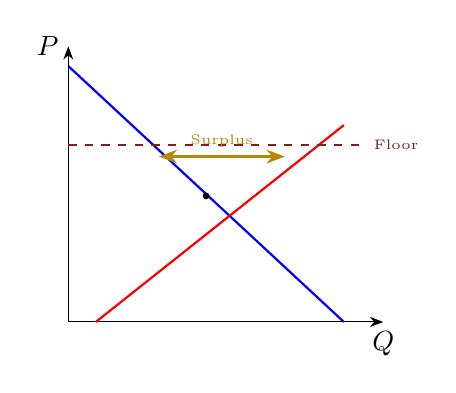
\begin{tikzpicture}[scale=0.5, >=Stealth]
  \draw[->] (0,0) -- (8,0) node[below] {$Q$};
  \draw[->] (0,0) -- (0,7) node[left] {$P$};
  \draw[thick, blue] (0, 6.5) -- (7, 0);
  \draw[thick, red] (0.7, 0) -- (7, 5);
  \draw[dashed, UoERed, thick] (0, 4.5) -- (7.5, 4.5)
    node[right, font=\tiny] {Floor};
  \filldraw (3.5, 3.2) circle (2pt);
  \draw[<->, UoEGold, thick] (2.3, 4.2) -- (5.5, 4.2);
  \node[above, font=\tiny, UoEGold] at (3.9, 4.2) {Surplus};
\end{tikzpicture}
\end{center}
\end{columns}
\end{frame}

\begin{frame}[fragile]{A Nonlinear Market: Why We Need Computers}
Real markets are rarely linear:
\vspace{0.3em}
\begin{align*}
  Q^D(P) &= \frac{500}{1 + 0.1\,P^{1.5}} \\[6pt]
  Q^S(P) &= 10 \ln(1 + P)
\end{align*}
\vspace{0.3em}
No algebraic solution exists --- but \texttt{fsolve} handles it:
\begin{lstlisting}
def excess_demand_nl(P):
    return 500 / (1 + 0.1*P**1.5) - 10*np.log(1 + P)

P_star_nl = fsolve(excess_demand_nl, x0=20)[0]
# P* = 22.61, Q* = 32.60
\end{lstlisting}
\vspace{0.3em}
The invisible hand works the same way whether the curves are straight lines
or complicated nonlinear functions.
\end{frame}

\begin{frame}[fragile]{Simulating the Invisible Hand}
Smith: the market price ``gravitates'' toward equilibrium.\\[6pt]
\textbf{Price adjustment rule:}
\[
  P_{t+1} = P_t + \lambda \cdot ED(P_t)
\]
\begin{lstlisting}
def simulate_market(P0, lam, T, ed_func):
    prices = np.empty(T)
    prices[0] = P0
    for t in range(1, T):
        prices[t] = prices[t-1] + lam * ed_func(prices[t-1])
    return prices
\end{lstlisting}
\vspace{0.3em}
\begin{itemize}
  \item Shortage ($ED > 0$) $\Rightarrow$ price rises
  \item Surplus ($ED < 0$) $\Rightarrow$ price falls
  \item $\lambda$ controls the speed of adjustment
\end{itemize}
\end{frame}

\begin{frame}{Convergence to Equilibrium}
\begin{center}
\begin{tikzpicture}[scale=0.7]
  \draw[->] (0,0) -- (10,0) node[below] {Time};
  \draw[->] (0,0) -- (0,6) node[left] {$P$};
  % Equilibrium line
  \draw[dashed, black] (0, 3.2) -- (10, 3.2);
  \node[left, font=\small] at (0, 3.2) {$P^*$};
  % Path from above
  \draw[thick, red] plot[smooth] coordinates
    {(0,5.5) (1,4.6) (2,4.0) (3,3.6) (4,3.4) (5,3.3) (6,3.22) (7,3.2)};
  \node[right, font=\small, red] at (7.1, 3.5) {Start high};
  % Path from below
  \draw[thick, blue] plot[smooth] coordinates
    {(0,0.8) (1,1.6) (2,2.2) (3,2.6) (4,2.9) (5,3.05) (6,3.15) (7,3.2)};
  \node[right, font=\small, blue] at (7.1, 2.9) {Start low};
\end{tikzpicture}
\end{center}
\vspace{0.5em}
No matter where the price starts, it converges to equilibrium.\\[4pt]
\textbf{The market corrects itself} --- shortages push prices up,
surpluses push them down.
\end{frame}

% -------------------------------------------------------------
\section{Part III --- Exercises \& Discussion}
% -------------------------------------------------------------

\begin{frame}{Exercise 1: A Tax on Oats}
The Scottish Parliament imposes a \textbf{per-unit tax} $\tau = 5$ shillings,
paid by sellers.
\vspace{0.5em}
\[
  Q^S_{\text{tax}}(P) = c + d(P - \tau)
\]
\vspace{0.3em}
\begin{enumerate}
  \item Define \texttt{supply\_tax(P, tau=5)} and a new excess demand function.
  \item Use \texttt{fsolve} to find the new equilibrium.
  \item Who bears more of the tax --- buyers or sellers?
  \item Plot old vs.\ new supply curves with both equilibria.
\end{enumerate}
\end{frame}

\begin{frame}{Exercise 2: The Corn Laws}
Two-country trade model (Britain vs.\ France):
\vspace{0.3em}
\begin{center}
\begin{tabular}{lcc}
\toprule
 & Britain & France \\
\midrule
Demand & $Q^D = 300 - 5P$ & $Q^D = 200 - 3P$ \\
Supply & $Q^S = 50 + 2P$  & $Q^S = 30 + 4P$ \\
\bottomrule
\end{tabular}
\end{center}
\vspace{0.5em}
\begin{enumerate}
  \item Find each country's autarky equilibrium price.
  \item Which country has the lower price? What does Smith predict?
  \item Find the world equilibrium price (sum of excess demands $= 0$).
  \item At the world price, who imports and who exports?
\end{enumerate}
\end{frame}

\begin{frame}{Exercise 3: Does the Starting Guess Matter?}
\begin{enumerate}
  \item Try the nonlinear excess demand with starting guesses\\
        $P_0 = 1, 10, 50, 100, 500$. Do all converge to the same root?
  \item Try the pathological function:
  \[
    ED(P) = \sin(P) - 0.1P + 1
  \]
  Multiple roots! Different starting guesses $\Rightarrow$ different solutions.
  \item Connection to Smith: is the ``natural price'' always unique?
\end{enumerate}
\vspace{0.5em}
\begin{alertblock}{Lesson}
Computational methods require care --- always check your results
and try multiple starting points.
\end{alertblock}
\end{frame}

% -------------------------------------------------------------
\section{Key Takeaways}
% -------------------------------------------------------------

\begin{frame}{What We Learned This Week}
\begin{enumerate}
  \item Adam Smith (1776) showed that \textbf{self-interested behaviour},
        channelled through markets, can produce socially beneficial outcomes.
  \item The \textbf{invisible hand} is the tendency of market prices
        to gravitate toward equilibrium.
  \item We can \textbf{compute} equilibria by finding roots of excess demand
        functions using \texttt{fsolve}.
  \item Government interventions (price floors, taxes) can be modelled
        and their welfare effects quantified.
  \item Numerical methods handle \textbf{nonlinear} markets where
        algebra fails.
\end{enumerate}
\end{frame}

\begin{frame}{Further Reading}
\begin{itemize}
  \item Smith, A. \textit{The Wealth of Nations} (1776), Book~I, Chs.~1--7.\\
        Free at \url{https://www.econlib.org/library/Smith/smWN.html}
  \item Heilbroner, R. \textit{The Worldly Philosophers}, Ch.~3.
  \item Broadie, A. \textit{The Scottish Enlightenment}.
  \item Phillipson, N. \textit{Adam Smith: An Enlightened Life}.
\end{itemize}
\vspace{1em}
\begin{center}
\textbf{Next week:} The Division of Labour and the Pin Factory ---\\
Smith's most famous example, and the logic of specialisation and trade.
\end{center}
\end{frame}

\end{document}
